% !TeX root = ../Project.tex
\section{Supporting Result Diagnostics}
\label{sec:results-supporting}

Figures~\ref{fig:appendix-reconstruction-examples} and~\ref{fig:appendix-reconstruction-failures} show additional whole-protein reconstructions and representative local failure modes.

\begin{figure}[H]
\centering
\captionsetup{font=small,skip=3pt}
\begin{minipage}[t]{0.48\linewidth}
  \centering
  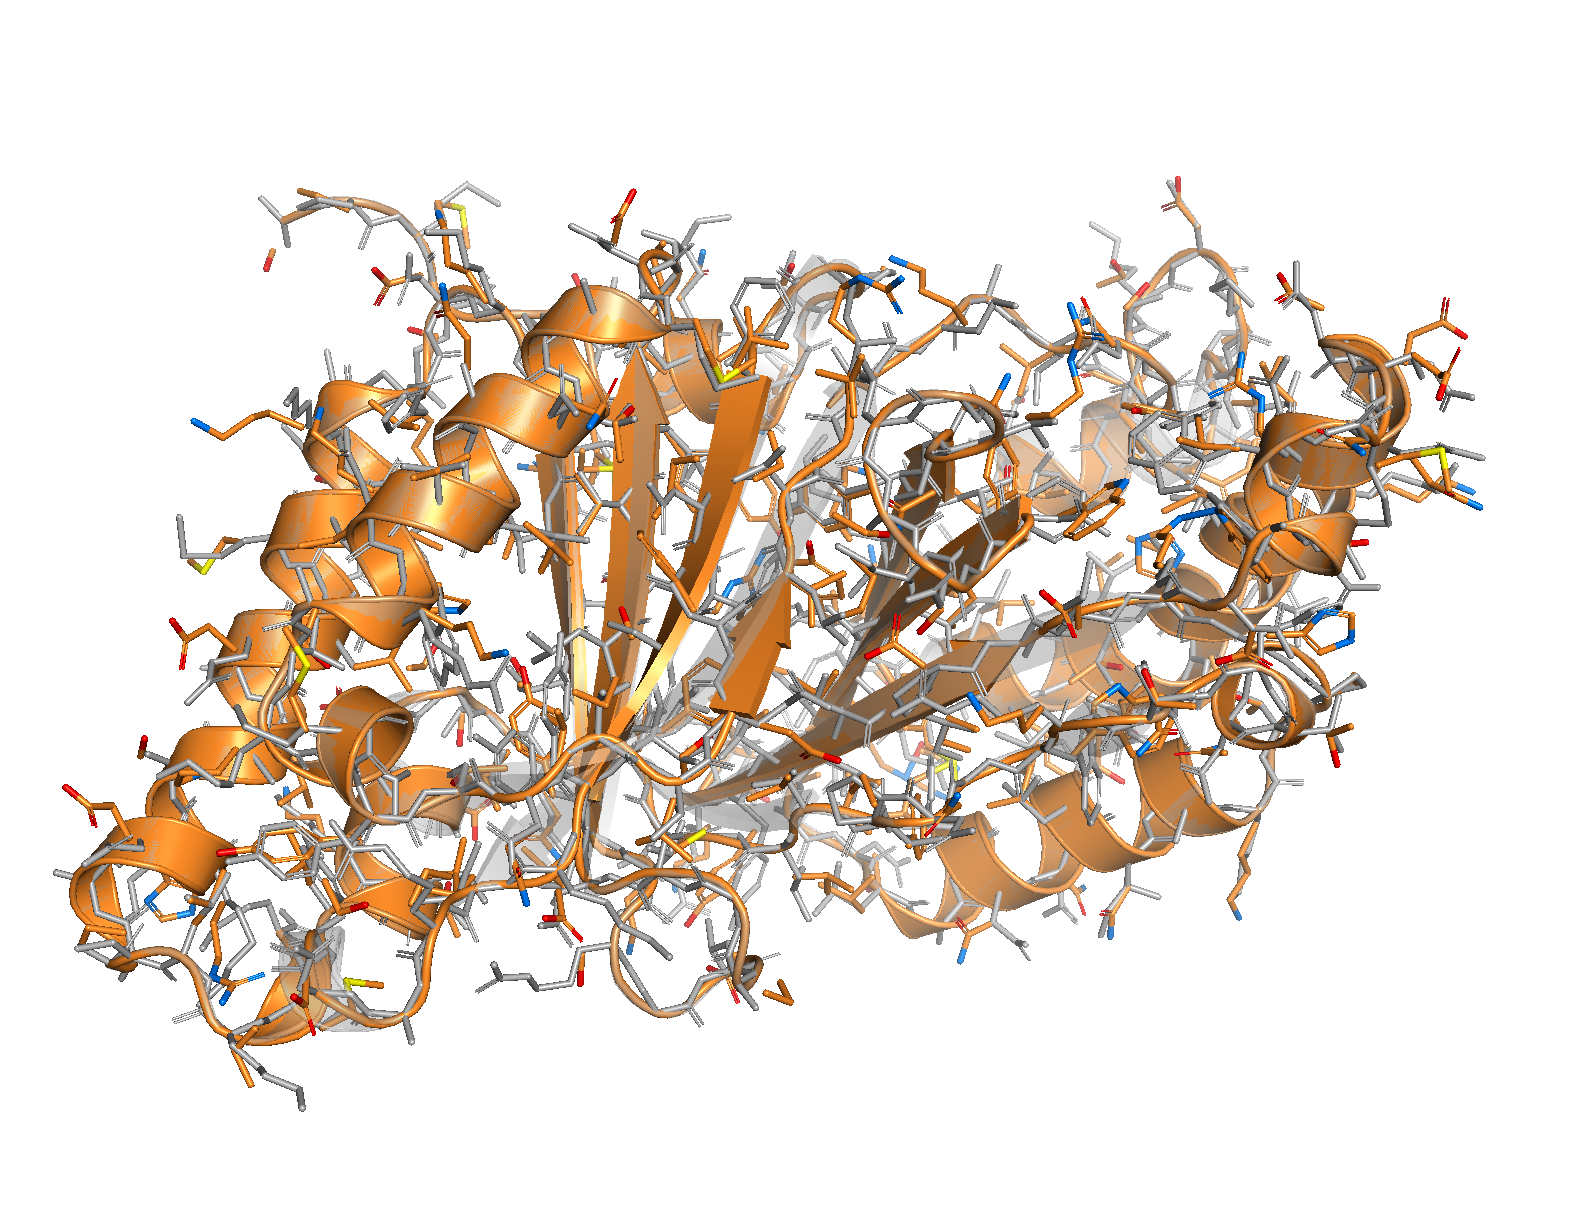
\includegraphics[height=0.14\textheight]{figures/protein_figures/5a13_G.png}\\[-2pt]
  \small (a) 5A13 chain G
\end{minipage}\hfill
\begin{minipage}[t]{0.48\linewidth}
  \centering
  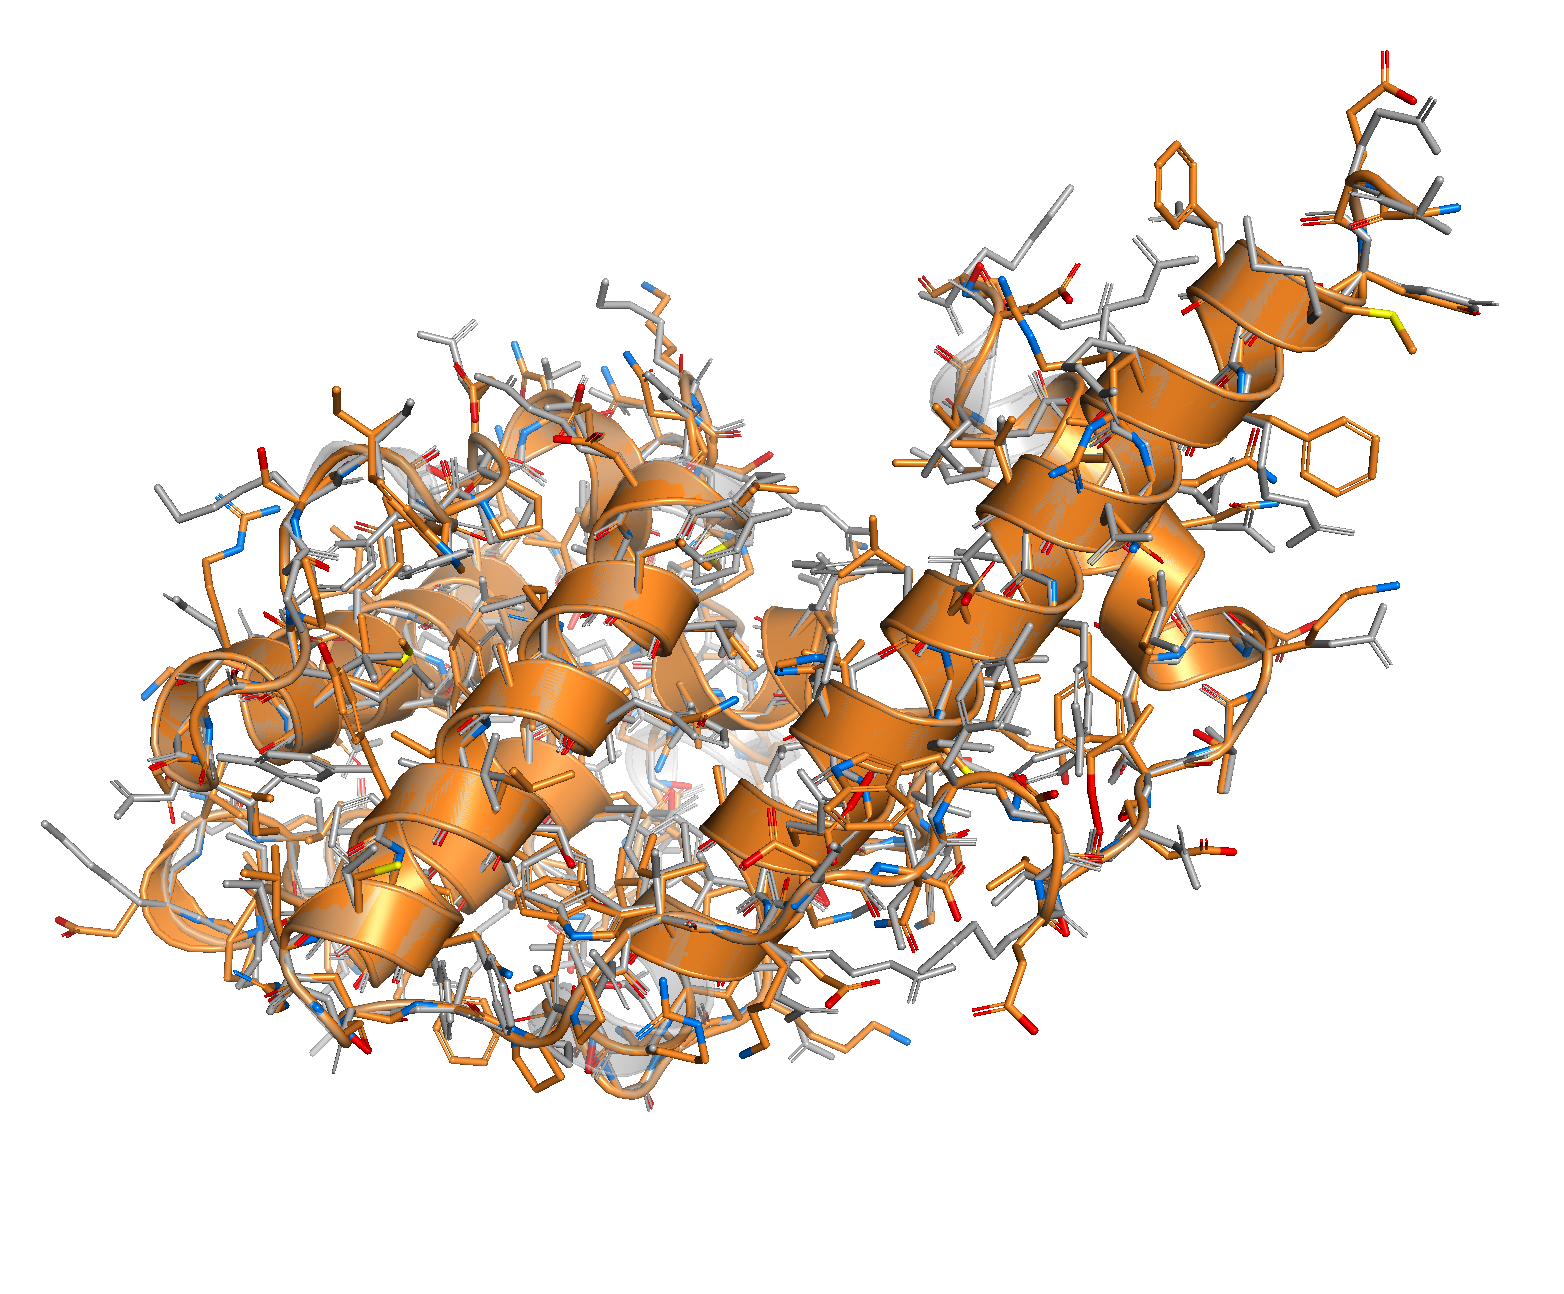
\includegraphics[height=0.14\textheight]{figures/protein_figures/5l0o_A.png}\\[-2pt]
  \small (b) 5L0O chain A
\end{minipage}

\vspace{2pt}
\begin{minipage}[t]{0.48\linewidth}
  \centering
  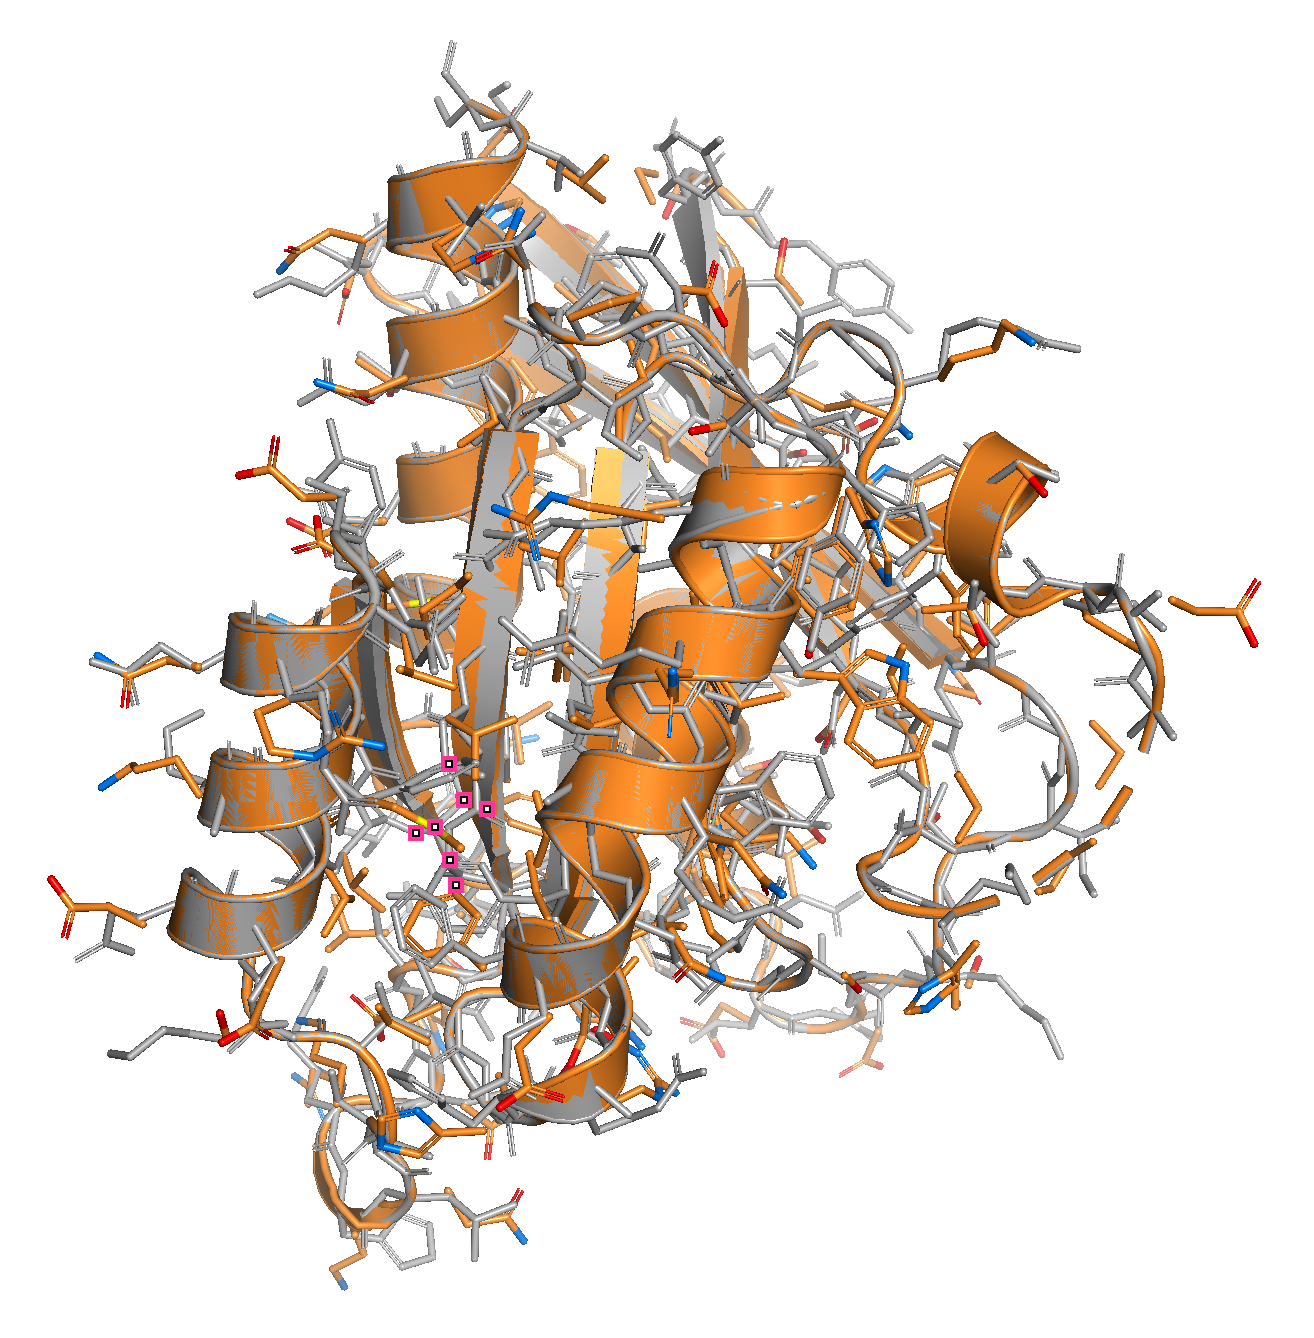
\includegraphics[height=0.14\textheight]{figures/protein_figures/5xr7_A.png}\\[-2pt]
  \small (c) 5XR7 chain A
\end{minipage}\hfill
\begin{minipage}[t]{0.48\linewidth}
  \centering
  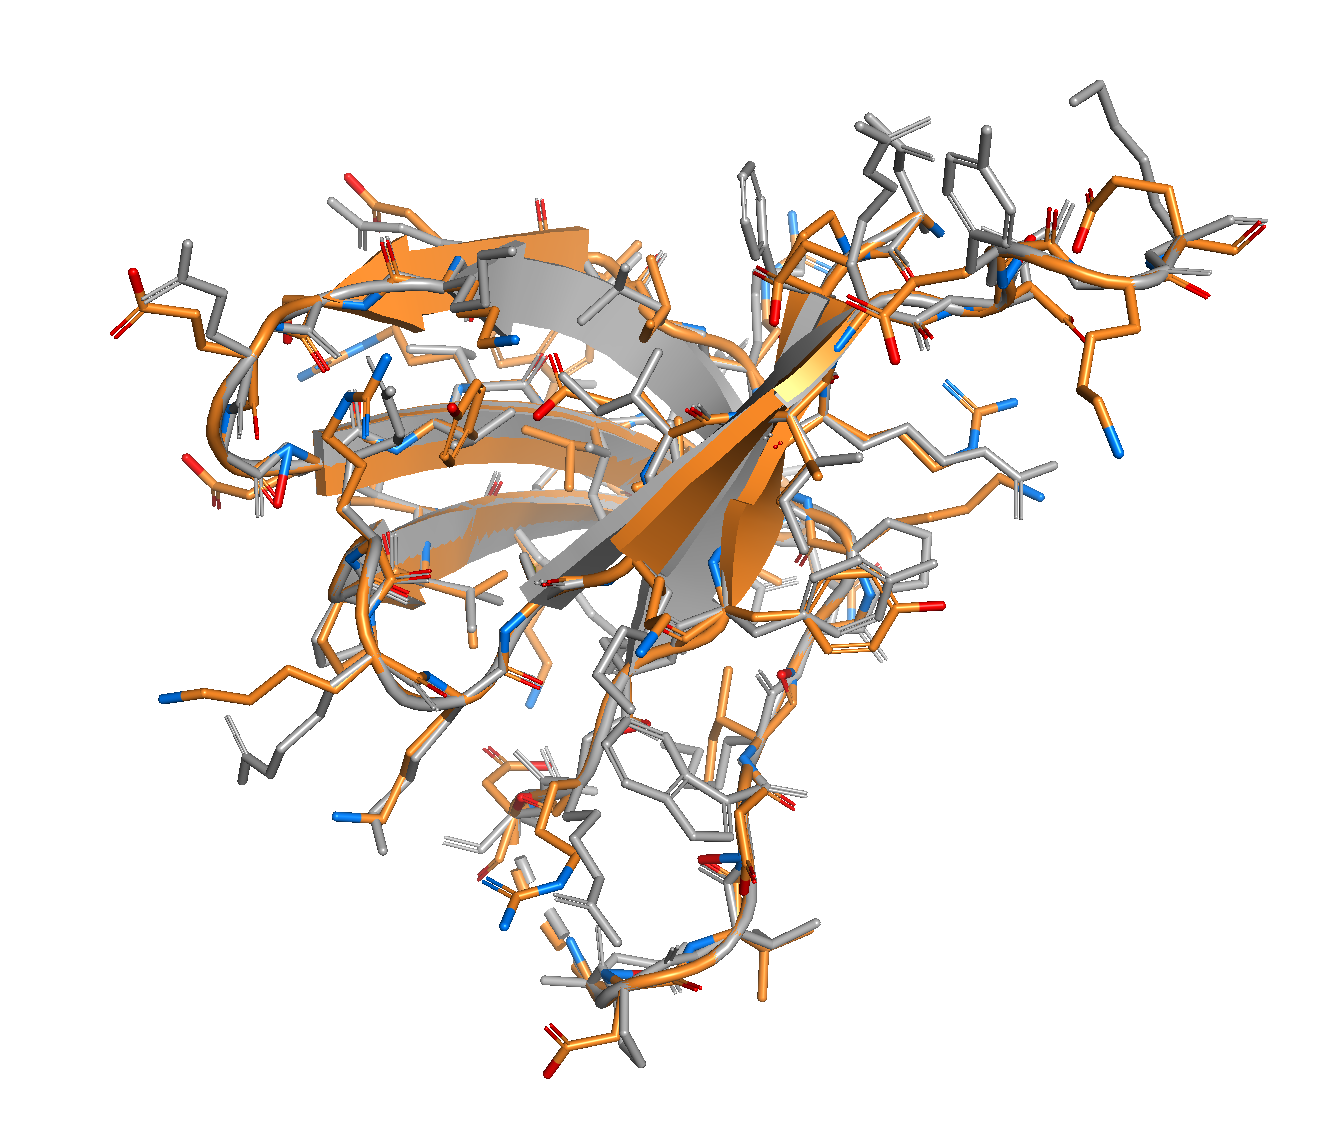
\includegraphics[height=0.14\textheight]{figures/protein_figures/8cbv_A.png}\\[-2pt]
  \small (d) 8CBV chain A
\end{minipage}
\caption{Whole-protein overlays of native structures in grey and postprocessed JEPA reconstructions in orange.}
\label{fig:appendix-reconstruction-examples}
\end{figure}

\begin{figure}[H]
\centering
\captionsetup{font=small,skip=3pt}
\begin{minipage}[t]{0.48\linewidth}
  \centering
  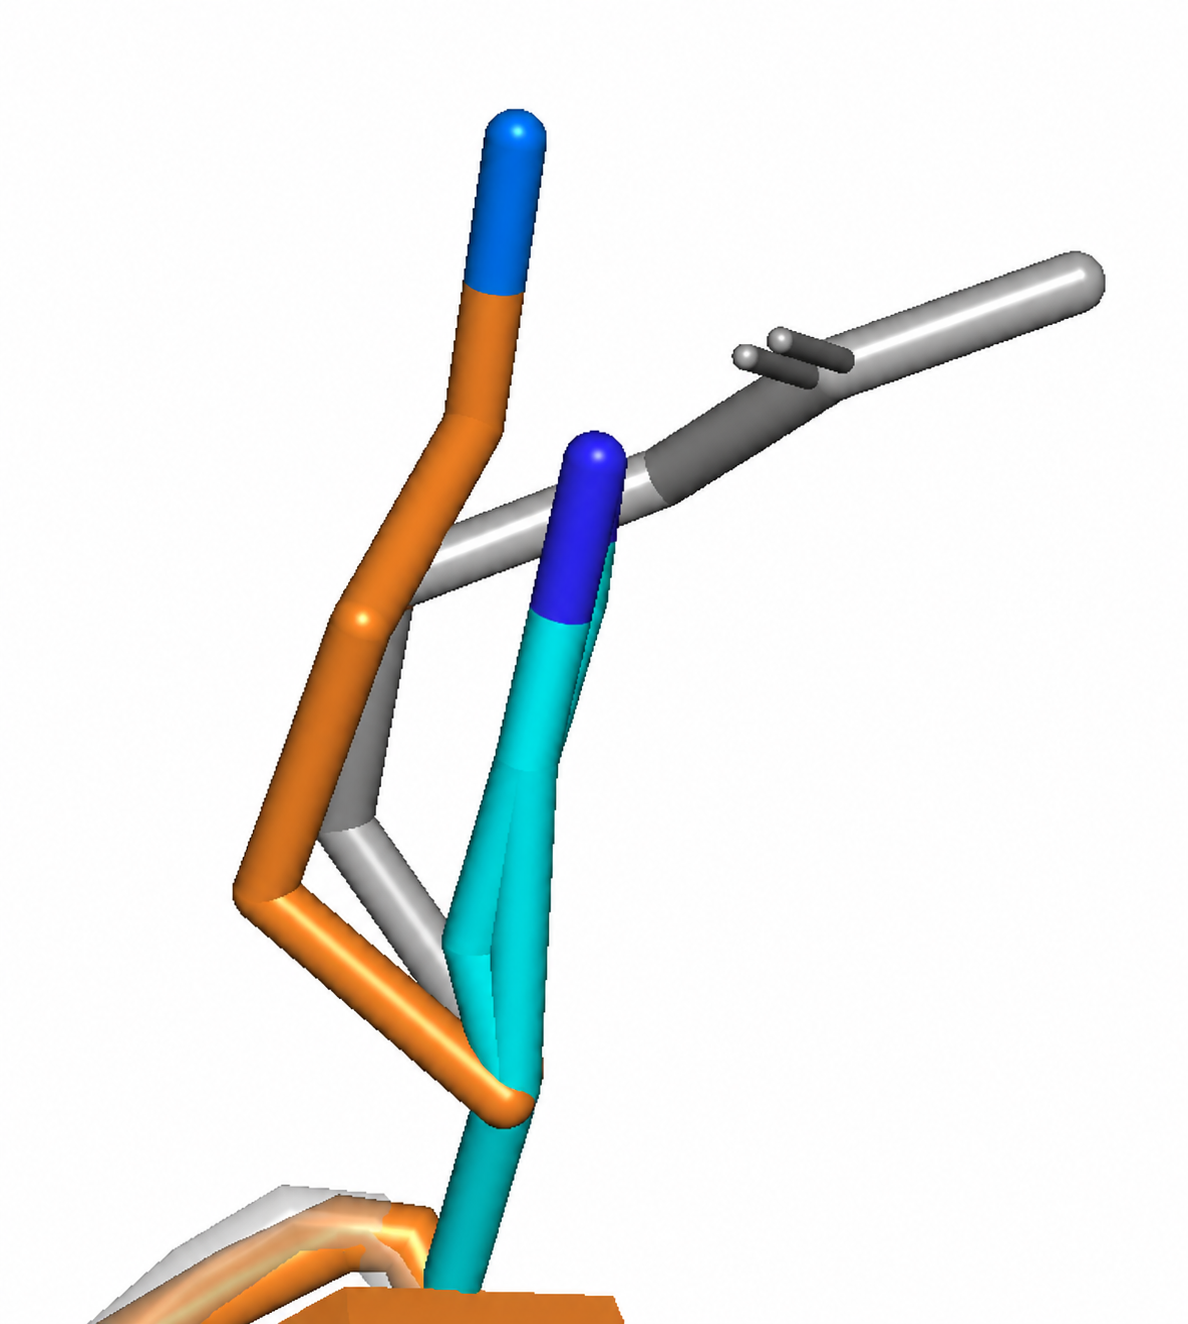
\includegraphics[height=0.14\textheight]{figures/protein_figures/fm1-clean.png}\\[-2pt]
  \small (a) Distorted bond geometry
\end{minipage}\hfill
\begin{minipage}[t]{0.48\linewidth}
  \centering
  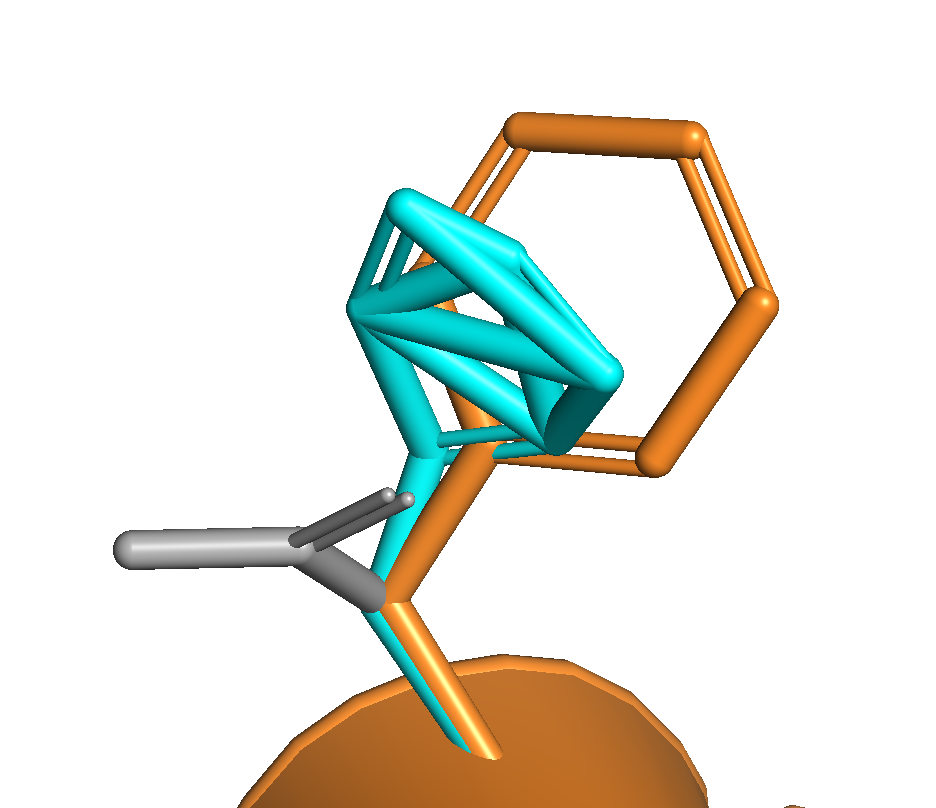
\includegraphics[height=0.14\textheight]{figures/protein_figures/fm2.png}\\[-2pt]
  \small (b) Overlapping side-chain atoms
\end{minipage}

\vspace{2pt}
\begin{minipage}[t]{0.48\linewidth}
  \centering
  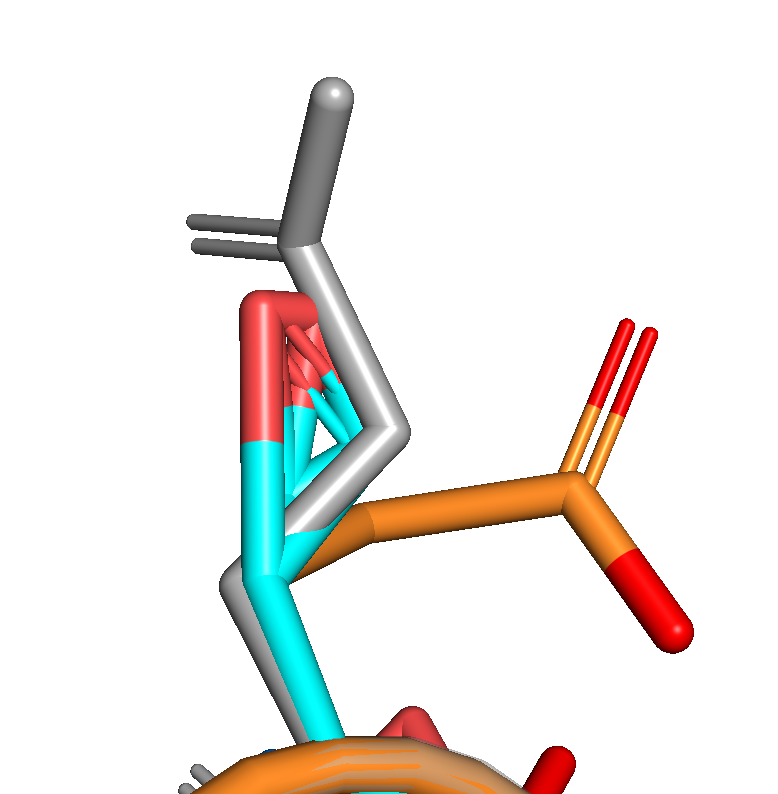
\includegraphics[height=0.14\textheight]{figures/protein_figures/fm3.png}\\[-2pt]
  \small (c) Misplaced side-chain atoms
\end{minipage}\hfill
\begin{minipage}[t]{0.48\linewidth}
  \centering
  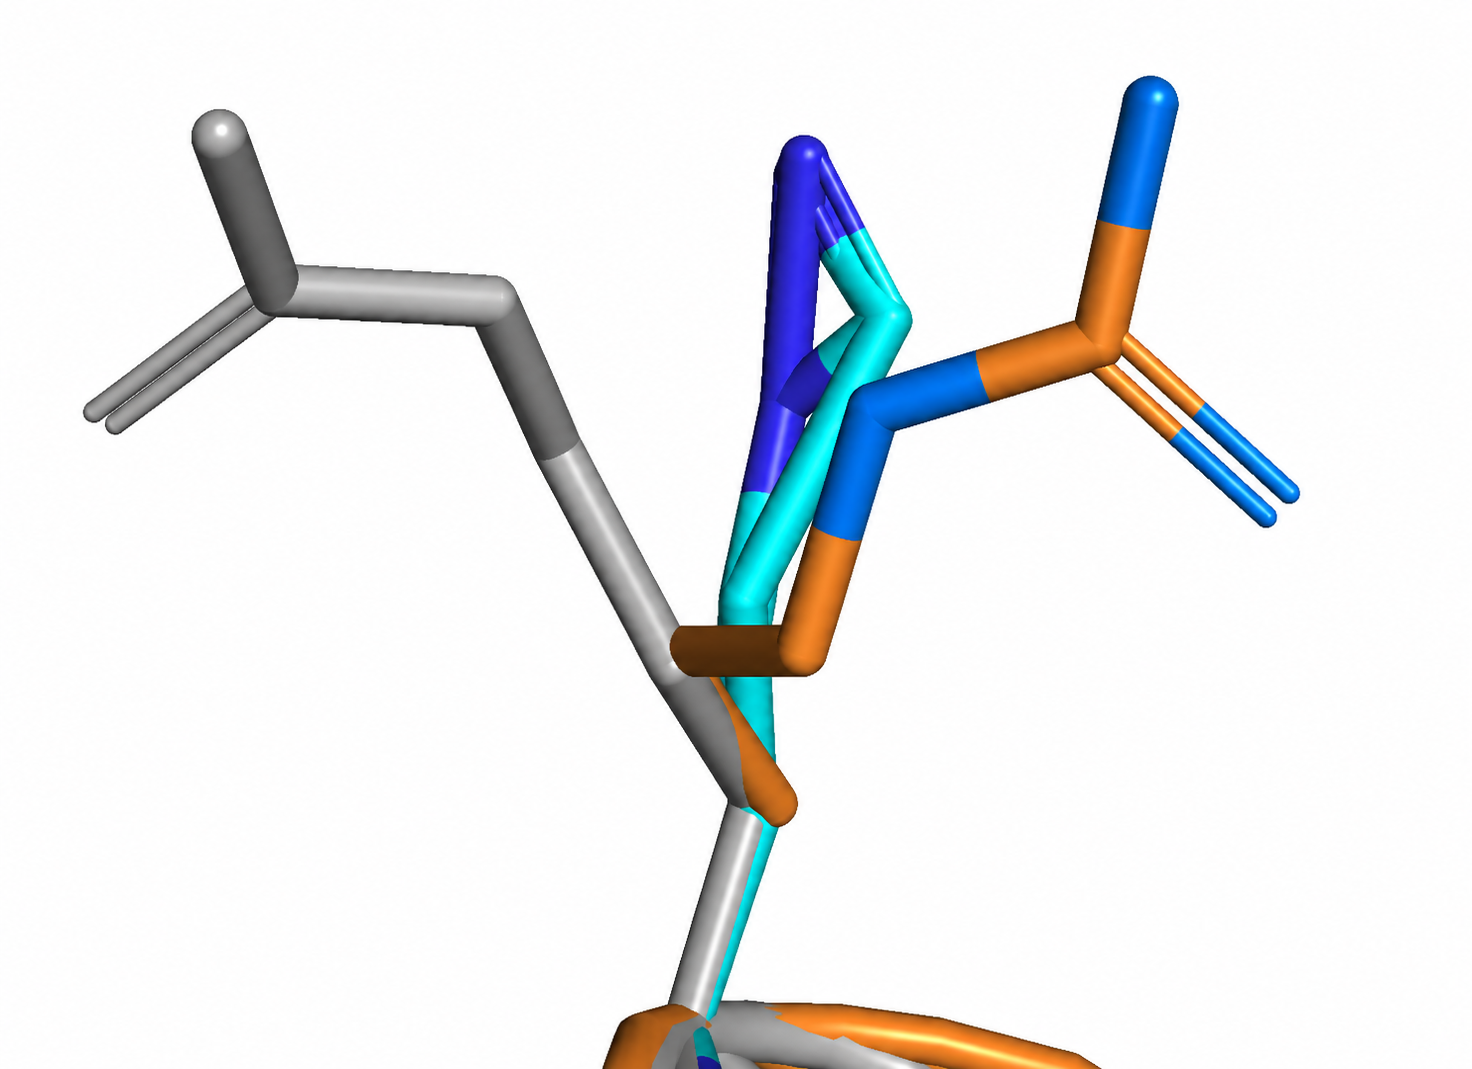
\includegraphics[height=0.14\textheight]{figures/protein_figures/fm4-clean.png}\\[-2pt]
  \small (d) Distorted local connection
\end{minipage}
\caption{Examples of local geometric failure modes. Native structures are grey, postprocessed JEPA predictions are orange, and direct decoder outputs are cyan.}
\label{fig:appendix-reconstruction-failures}
\end{figure}
